\documentclass[border=10pt]{standalone}
\usepackage[european]{circuitikz}
\begin{document}
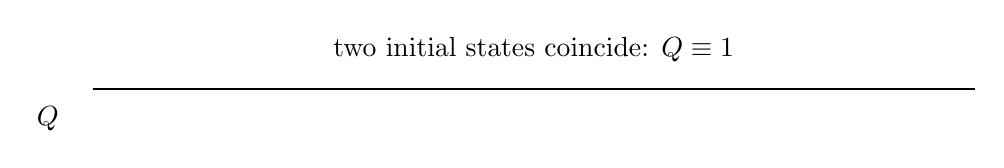
\begin{tikzpicture}[x=1cm, y=1cm, font=\normalsize, line width=0.8pt]
  % 8.1 答案波形：两种初态(Q=0/Q=1)重合，Q 从原点起恒 1。
  % 横轴 0–100%，与 fig-8-01 同刻度（总宽 11.2cm，每 1% = 0.112cm）。
  \def\pp{0.112}
  \def\hi{0.75}
  \def\total{11.2}

  \node[anchor=east] at (-0.3,\hi/2) {$Q$};
  \draw (0,\hi) -- (\total,\hi);
  \node[anchor=south] at (\total/2,\hi+0.22) {two initial states coincide: $Q\equiv1$};

\end{tikzpicture}
\end{document}
